\graphicspath{{chapters/06_images/}}
\chapter{Biocompatibility}

\section{Introduction}
Biocompatibility is an essential aspect to take into consideration for the specification of the medical device that is being designed.
Before building a scaffold or a biological device its time, location and individual in which it will be used need to be defined.
A scaffold to be useful should activate specific cellular function and reflect and exploit the different mechanical and chemical properties of the tissue in which it will be implanted.
Because of this a scaffold it's designed taking into account the specific region in which it will be implanted considering the cell population and kind of injury among other parameters.
Cells are the building blocks of biology and they can read the information coming from the external environment.
Specific gene expression is activated in cells given external signalling molecules.
This makes it evident that the environment reaches the cell through chemical and mechanical stimuli.
Because of this scaffold are not self-sufficient entities: they are bioactive and need to collaborate with environment, cells and the extracellular matrix to perform their function.

	\subsection{Parameters defining biological outcome}
	The biological outcome that will be obtained then depends on a list of parameters which, once defined allow for the creation of a scaffold capable of regenerating the injured tissue.
	This parameters are:

	\begin{multicols}{2}
		\begin{description}
		\item[Porosity] is extremely important for cell migration.
			The material should be 3D for the cells, meaning that the scaffold should allow and promote cell adhesion, growth and migration.
		\item[Mechanical properties] are different for each tissue, the scaffold should both resist physical stress and provide the correct stimulus that the cells need to grow, adhere, migrate and differentiate.
		\item[Surface] modification is often referred to the functionalization of the scaffold through the addition of proteins or sequence of aminoacids to increase adherence.
		\item[Antibiotic/antiviral] drugs release system, to control chronic inflammation and possible infections.
		\item[Surface topography] may be smooth or rough for example.
		\end{description}
	\end{multicols}

\section{Guided tissue regeneration}
\begin{figure}[ht]
\centering
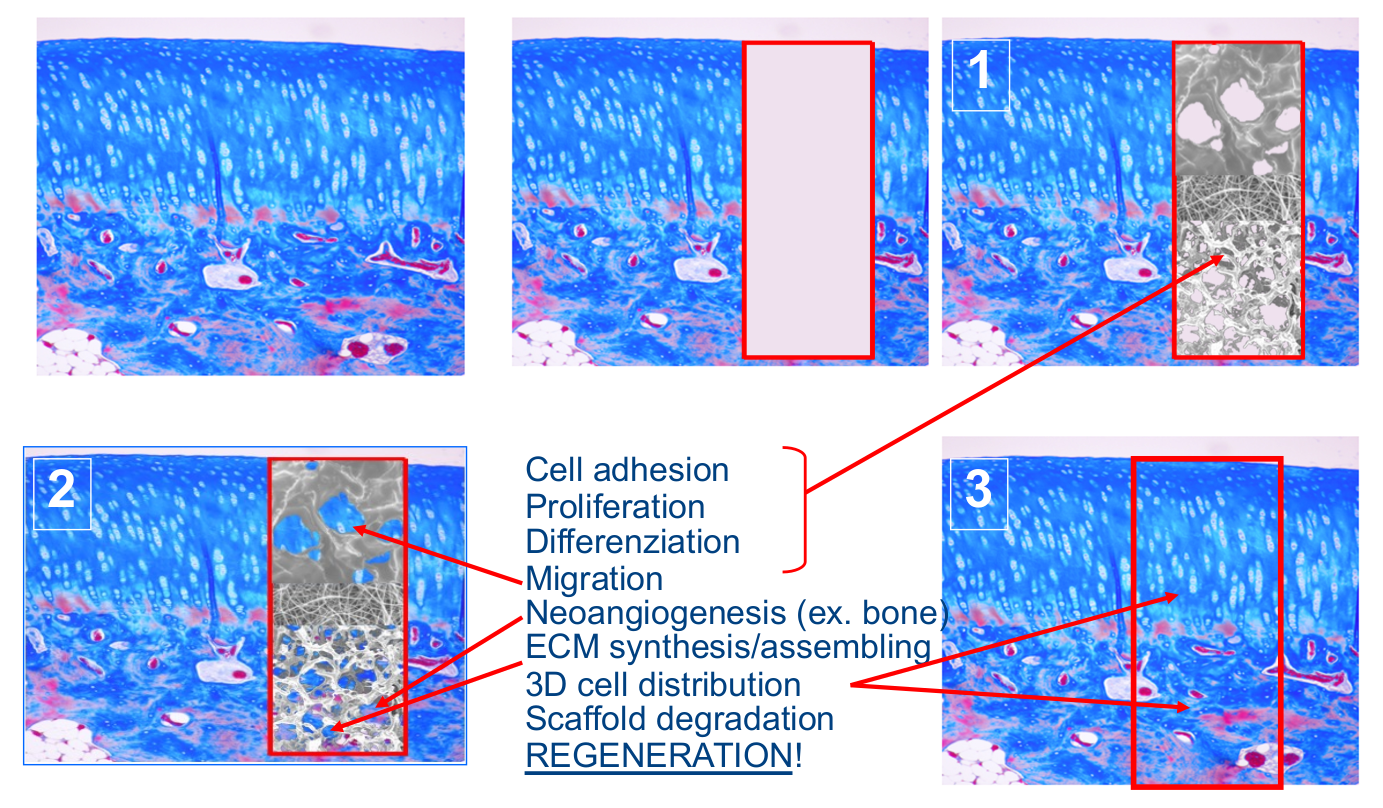
\includegraphics[width=0.5\textwidth]{cartilage.png}
\caption{\label{fig:cartilage}}
\end{figure}
In the figure we can see articular cartilage, an intermidiate zone and bone. These three different tissues present differences in vasculartion, cell organization (in cartilage cells live in lacuna, where migration and proliferation are downregulated) and innervation.
\\
If the damage reaches the bone (which happens most of the times, because the cartilge does not have innervation, while bone does), the scaffold needs to account for different types of tissue. A multicomponent scaffold is designed, something that upregulates angiogenesis in the bone and downregulates it in the cartilage, that has high resistance to mechanical stimulations (cartilage has more water, material reaching water with hydrofilic properties). It should also provide for an enviroment for osteoblasts, lacunae for cartilage cells, space for nerves, vascularity and migration. It also needs to have different degradation times.
\\
The next step is check the biocompatibility, which will have an impact on cell adhesion, proliferation, differentiation, and also migration; on neoangiogenesis (spefic function) etc. Difference between regeration and repair (no/presence of scar tissue).

\section{The principles of tissue engineering}
\begin{figure}[ht]
\centering
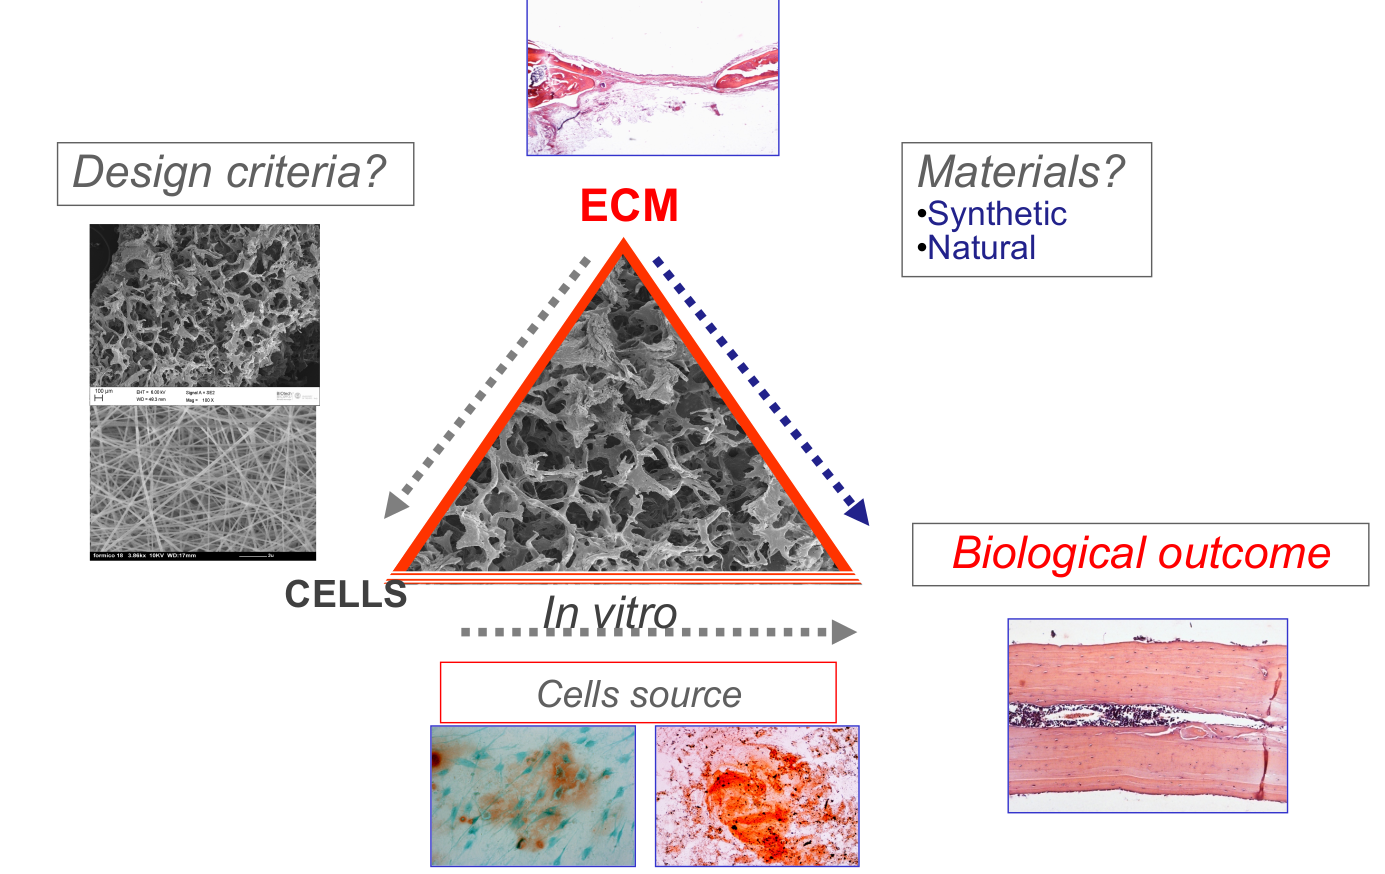
\includegraphics[width=0.5\textwidth]{triangolo.png}
\caption{\label{fig:triangle}}
\end{figure}

A tissue engineering process is composed by three steps:

\begin{multicols}{3}
	\begin{itemize}
		\item Design.
		\item Material choice.
		\item In vitro and in vivo testing.
	\end{itemize}
\end{multicols}

Tissue engineering implements a multidisciplinary strategy and the advance in materials' science and biology drastically improve the success of scaffold application.
Just consider how much the progressive knowledge in biology incremented the one in biocompatibility.
For example, M1 and M2 macrophages were only discovered in 2000.
But also the invention of polymers that can change their activity based on the environment (thermo/ph responsive), instructional (functionalization, e.g. with peptides that can control the cells' fate) and that can have specific mechanical strength and function (mechanical signalling).
In particular, the materials that can satisfy those requirements are considered 4th generation "biological regenerative biomaterials".
\\
Biomaterial need to be stable and inert in the beginning to be able to deliver drugs, to be used to print organ and used for cell therapies.
The hope for the future is to develop also diagnostic systems and to implant electronic devices, but one thing must always be present: biocompatibility.

	\subsection{Biocompatibility: a definition}
	At first, a material is biocompatible when inert, a ghost in the body: "the total absence of interaction between the material and the tissues".
	The minimal reaction to the foreign body was preferred, meaning no (or low) inflammatory reaction, no immuno-response.
	Definition focused on the body reaction to the implant and what was required was simply the chemical stability by the time.
	\\
	\begin{figure}[ht]
\centering
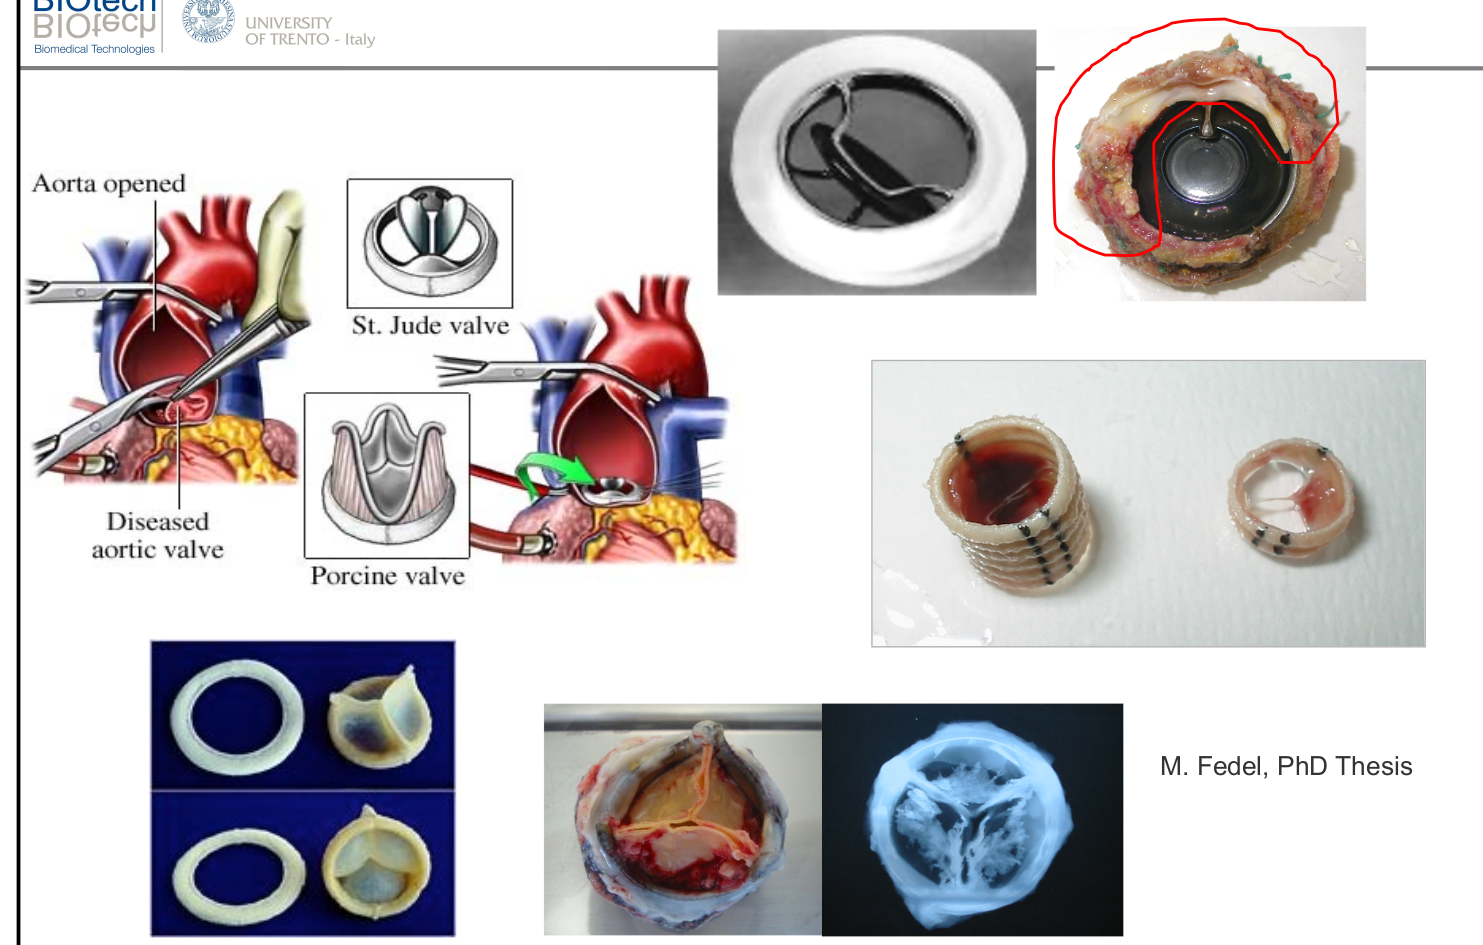
\includegraphics[width=0.5\textwidth]{valves.png}
\caption{\label{fig:valves}}
\end{figure}
	People however changed idea based on what they discovered after seeing what happened in the body after some time after implantation.
	Heart valve made of titanium and polyester failed because around the plastic layer the body built a very thick scar tissue and the valve could not open any more.
	The same valve in another patient induced trombosis.
	This first valve was treated with anticouagulants.
	The context of implantation is extremely important.
	A biological heart valve was harvested from pigs, but it failed because of calcification which rendered the valve unable to close.
	All the material induce a biological reaction.
	No material is completely inert, because our antibodies can recognize anything that is not "self".
	\\
	The concept of biocompatibility was revised: the ability of a material to perform a specific application causing an appropriate host response in a specific application” (1987).
	\\
	\begin{figure}[ht]
\centering
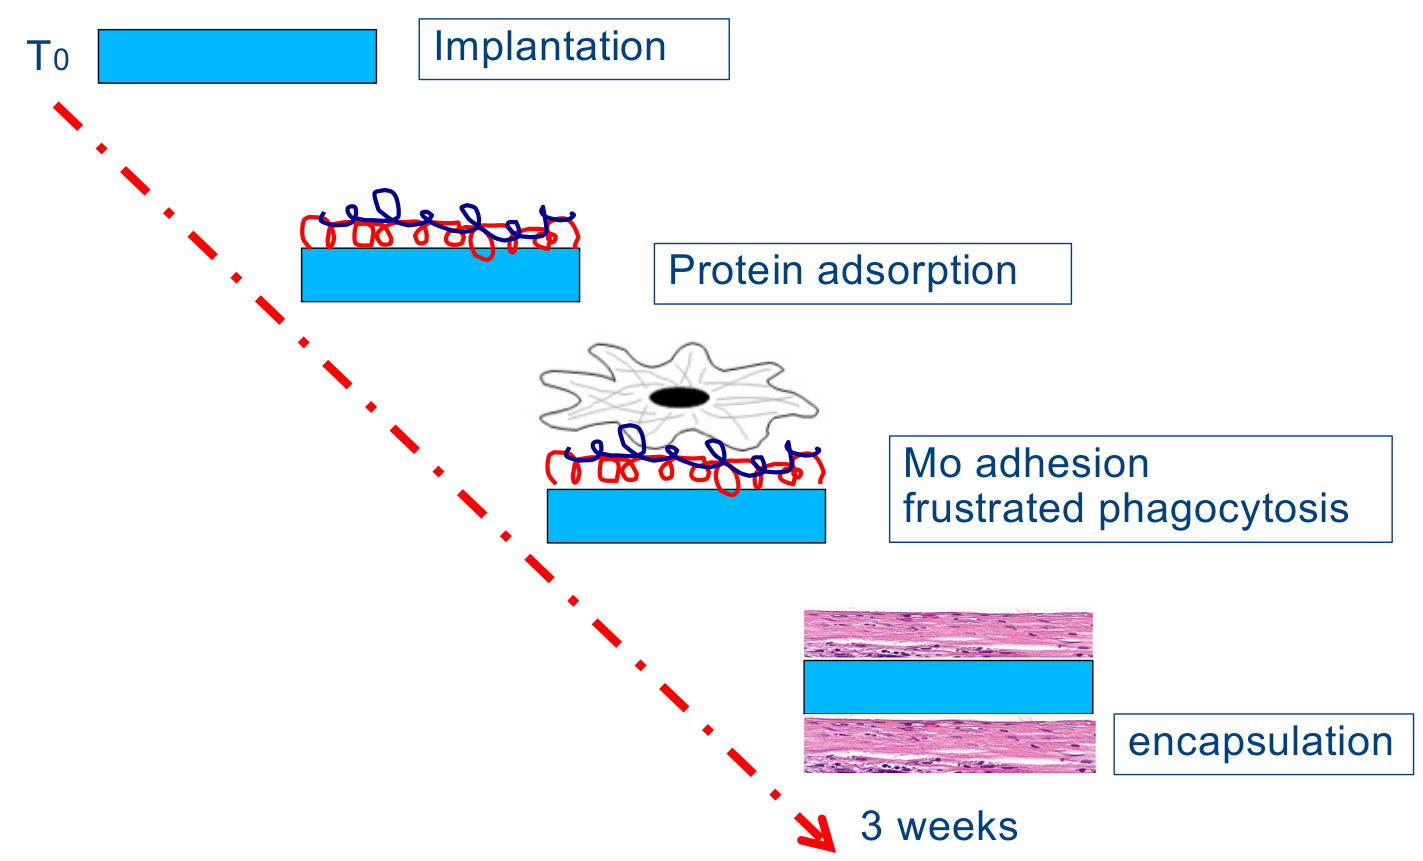
\includegraphics[width=0.5\textwidth]{fbrx.png}
\caption{\label{fig:matrixome}}
\end{figure}
	We can take as an example FBRx (cos'è?????), a non porous scaffold material.
	Depending on the chemistry of the material a specific protein adsorption is activated and subsequently an immune response.
	But if the material is not degradable, the macrophages start to coat the foreign body with scar tissue.
	At this point the reaction is finished.
	If the scaffold degrades eventually we will have an empty bag.
	Just by changing the porosity the scar tissue is reduced and regeneration is promoted.
	\\
	Injectable gels (hydrogel) are useful when filling cavities, becomes scaffold and supply for a scaffold for cells to migrate to.
	\\
	Take home lesson: scaffold should be tissue-organ dependent, defined situation, specifically react with the tissue (induce activation of cellular function to heal in a specific environment), material degradation.

	\subsection{Re-evaluation of the biocompatibility concept}
	Some factors led to the redefinition of the concept of biocompatibiliy, as for the scaffold is not enough to simply "exists":

	\begin{multicols}{2}
		\begin{itemize}
			\item Response to specific materials could vary from one application site to another (tissue-organ dependent) and not just on the material characteristics but it should also defined the situation in which the material is used (pathology, function).
			\item An increasing number of applications require that the material specifically react with the tissues rather than be ignored by them.
				Some applications required that the material degrade over time in the body rather than remain indefinitely.
			\item
		\end{itemize}
	\end{multicols}

	Most advance concept: biocompatibility is not a material's property but a system's property. It cannot be defined without considering the context.

\section{The complexity of the biocompatible system}
\begin{figure}[ht]
\centering
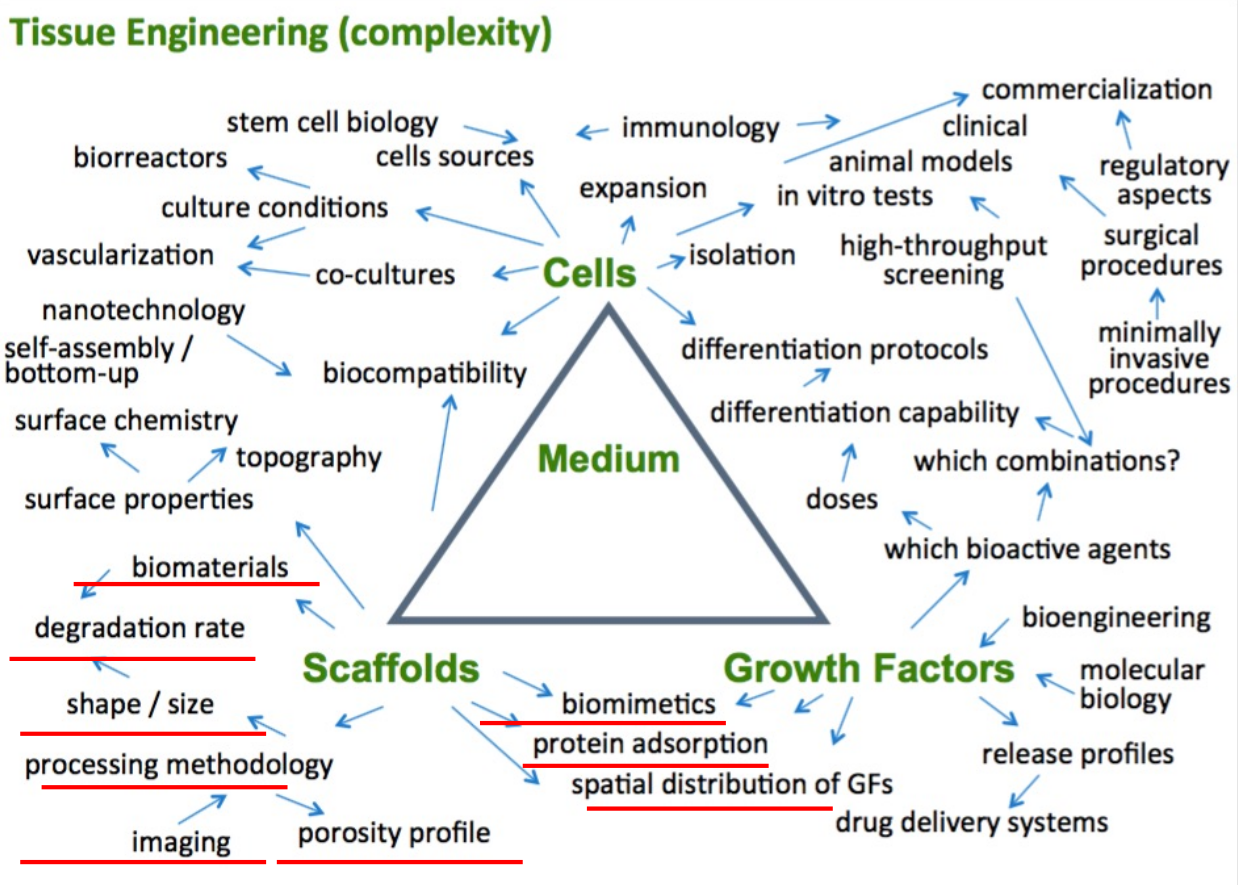
\includegraphics[width=0.8\textwidth]{piramide_completa.png}
\caption{\label{fig:complete_pyramid}}
\end{figure}
Tissue engineering as a triangle: it seems easy with only three actors.
Each one has many possibilities!
\\
For a scaffold to be biocompatible the following steps must be followed:

\begin{multicols}{2}
	\begin{itemize}
		\item Determination of native tissue-organ.
		\item From in vitro to in vivo (from smaller to bigger animals, that depending on the biological problem).
		\item At this point we need to define the surgical model and finally we move to clinical trials.
		\item In addition, for in vitro test now bioreactors are used, because we don't want steady conditions but we want mechanical stimuli (the perfusion provides stress but also washes away cell residues).
	\end{itemize}
\end{multicols}

	\subsection{ECM molecules production: effect of the mechanical stimuli}
	\begin{figure}[ht]
\centering
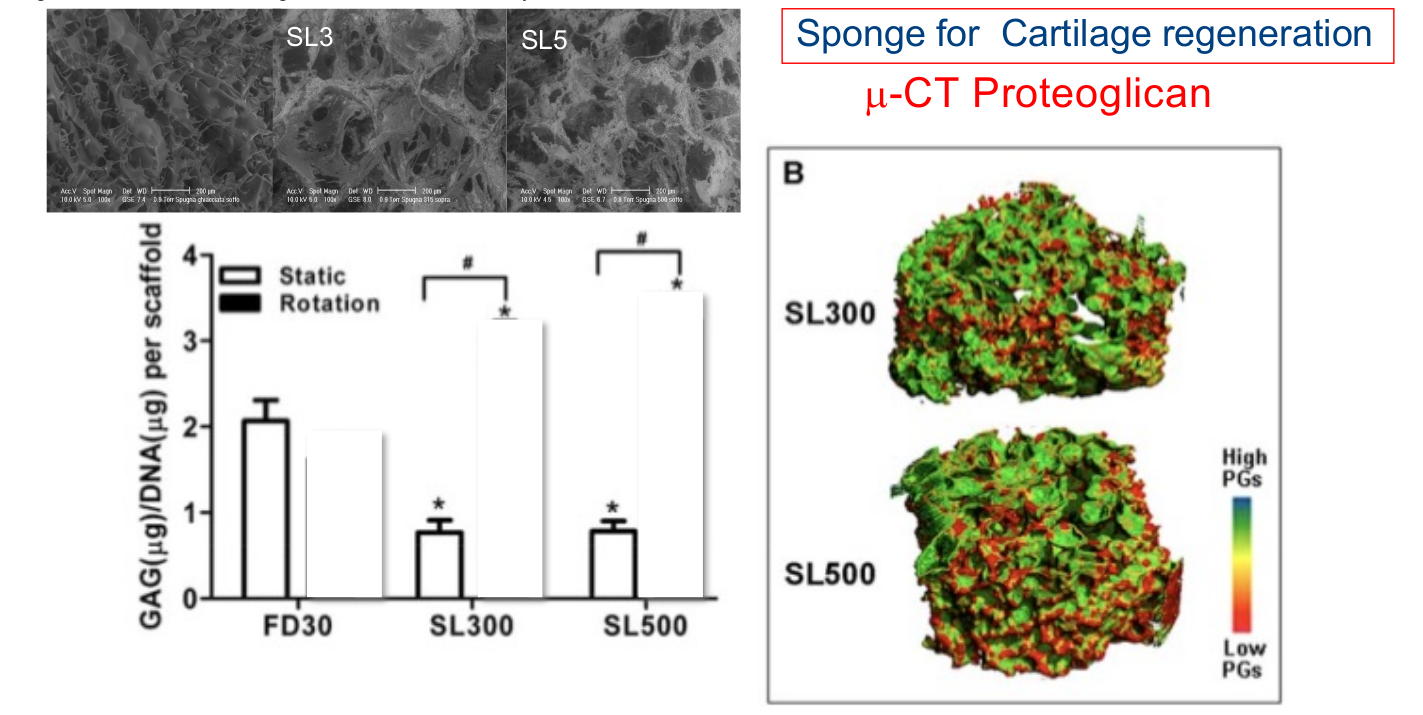
\includegraphics[width=0.5\textwidth]{sponge.png}
\caption{\label{fig:matrixome}}
\end{figure}
	Different sponge-like scaffolds were produced with different properties (like porosity) for cartilage regeneration.
	The quality of GAG (mainly into the ECM of cartilage) was assessed.
	In addition, microCT to see where the GAG is and the sponges are completely infiltrated with it.
	SL500 had a lot of green (GAG) but only on the outside.
	What happens if the devices undergoes a mechanical stress similar to the biological situations? We get the exact contrary! Just by changing from a static to a perfusion situation.
	By changing the environment we ultimately change integrins and biological performances.
	In perfusion, the integrins were upregulated! Integrins are transmembrane proteins: portion inside and outside and are important so that scaffolds are able to talk to cells, instructive behaviour.
	Cells are extremely sensitive.
	In the very first case the in vitro model was not well designed.
	We must perform extensive and well thought tests before moving to the application.
